% Created 2022-10-07 Fri 05:23
% Intended LaTeX compiler: pdflatex
\documentclass[12pt]{article}
\usepackage[utf8]{inputenc}
\usepackage[T1]{fontenc}
\usepackage{graphicx}
\usepackage{longtable}
\usepackage{wrapfig}
\usepackage{rotating}
\usepackage[normalem]{ulem}
\usepackage{amsmath}
\usepackage{amssymb}
\usepackage{capt-of}
\usepackage{hyperref}
\usepackage{fourier}
\usepackage{placeins}
\usepackage{authblk}


% authors
\author[1]{Peter~J.~Dodd}
\author[2]{C.~Finn~McQuaid}
\author[3]{Prasada~Rao}
\author[4]{Ibrahim~Abubakar}
\author[5]{Nim~Arinaminpathy}
\author[2]{Anna~Carnegie}
\author[6]{Frank~Cobelens}
\author[7]{David~Dowdy}
\author[8]{Kathy~Fiekert}
\author[9]{Alison~Grant}
\author[10]{Jing~Wu}
\author[11]{Faith~Nekabari~Nfii}
\author[12]{Nabila~Shaikh}
\author[2]{Rein~M~G~J~Houben}
\author[2]{Richard~White}

\affil[1]{School of Health and Related Research, University of Sheffield, Sheffield, UK}
\affil[2]{TB Modelling Group, TB Centre, London School of Hygiene \&Tropical Medicine, London,
  UK}
\affil[3]{Former Health Secretary, Government of India}
\affil[4]{University College London, UK}
\affil[5]{MRC Centre for Global Infectious Disease Analysis; and the Abdul Latif Jameel Institute
  for Disease and Emergency Analytics, School of Public Health, Imperial College London}
\affil[6]{The Amsterdam Institute for Global Health and Development, Netherlands}
\affil[7]{Johns Hopkins Bloomberg School of Public Health, USA}
\affil[8]{KNCV Tuberculosis Foundation, Netherlands}
\affil[9]{TB Centre, London School of Hygiene \&Tropical Medicine, London, UK; Africa Health
  Research Institute, South Africa}
\affil[10]{Center for Chronic Diseases Prevention and Control, China CDC, China}
\affil[11]{Africa Union-Africa Centres for Disease Control and Prevention}
\affil[12]{Sanofi, UK}

\date{}
\title{Improving the quality of the Institute for Health Metrics
  and Evaluation's Global Burden of Disease tuberculosis estimates: Appendix}
\hypersetup{
 pdfauthor={Author list},
 pdftitle={Appendix for IHME TB evaluation},
 pdfkeywords={},
 pdfsubject={},
 pdfcreator={Emacs 28.2 (Org mode 9.5.5)}, 
 pdflang={English}}
\begin{document}


\renewcommand{\Affilfont}{\footnotesize}
\renewcommand{\Authfont}{\normalsize}
\renewcommand\Authands{, }

\maketitle
% \tableofcontents

\newpage

\listoffigures

\newpage

\section*{Preamble}
\label{sec:orga0b5156}

The figures are generated with
publicly available data from WHO and IHME's Global Burden of Disease Collaborative
Network Global Burden of Disease Study 2019 (GBD 2019). They are available from:

\begin{itemize}
\item \url{https://www.who.int/teams/global-tuberculosis-programme/data}
\item \url{https://vizhub.healthdata.org/gbd-results/},
\end{itemize}
and are also included in the GitHub repository:

\begin{itemize}
\item \url{https://github.com/petedodd/ihmexplore}
\end{itemize}
for this article, which includes
the R code for analysis \& visualisation.

Some plots use ISO3 codes to refer to countries, which are provided on the next
page for reference.

\subsubsection*{Panel membership}
Prasada Rao Jvr (panel co-lead; former Special Envoy of UN Secretary General, India),
Richard White (panel co-lead; LSHTM, UK),  Faith Nekabari Nfii (Public
Health Specialist, Africa Union-Africa Centres for Disease Control and
Prevention), Pete Dodd (The University of Sheffield, UK),
Michael Klag (Dean Emeritus, Johns Hopkins Bloomberg School of Public Health, US).


The panel was supported by the Secretariat of the Global Burden of Disease
Independent Advisory Committee (GBD IAC) represented by Edmond Ng (Senior
Statistical Analyst), and Nabila Shaikh (Research Assistant, LSHTM).


\subsubsection*{Expert group membership}

Jing Wu (China CDC, China), Leigh Johnson (University of Cape Town, Sout
Africa), Ibrahim Abubakar (University College London, UK), Nim Arinaminpathy (Imperial College,
UK), Frank Cobelens (The Amsterdam Institute for Global Health and Development, Netherlands),
David Dowdy (Johns Hopkins Bloomberg School of Public Health, US), Kathy Fiekert
(KNCV, Netherlands), Philippe Glaziou (WHO, Switzerland),
Alison Grant (LSHTM, UK), Rein Houben (LSHTM, UK), Joshua Salomon (Stanford University, US)


\begin{table}[]
  \centering
\begin{tabular}{|l|l|}
\hline
\textbf{iso3} & \textbf{country name}                 \\ \hline
AGO           & Angola                                \\ \hline
BGD           & Bangladesh                            \\ \hline
BRA           & Brazil                                \\ \hline
KHM           & Cambodia                              \\ \hline
CAF           & Central African Republic              \\ \hline
CHN           & China                                 \\ \hline
COG           & Congo                                 \\ \hline
PRK           & Democratic People's Republic of Korea \\ \hline
COD           & Democratic Republic of the Congo      \\ \hline
ETH           & Ethiopia                              \\ \hline
IND           & India                                 \\ \hline
IDN           & Indonesia                             \\ \hline
KEN           & Kenya                                 \\ \hline
LSO           & Lesotho                               \\ \hline
LBR           & Liberia                               \\ \hline
MOZ           & Mozambique                            \\ \hline
MMR           & Myanmar                               \\ \hline
NAM           & Namibia                               \\ \hline
NGA           & Nigeria                               \\ \hline
PAK           & Pakistan                              \\ \hline
PNG           & Papua New Guinea                      \\ \hline
PHL           & Philippines                           \\ \hline
RUS           & Russian Federation                    \\ \hline
SLE           & Sierra Leone                          \\ \hline
ZAF           & South Africa                          \\ \hline
THA           & Thailand                              \\ \hline
TZA           & United Republic of Tanzania           \\ \hline
VNM           & Viet Nam                              \\ \hline
ZMB           & Zambia                                \\ \hline
ZWE           & Zimbabwe                              \\ \hline
\end{tabular}
\caption{Key of ISO3 codes and country names}
\end{table}


\begin{figure}
  \centering
  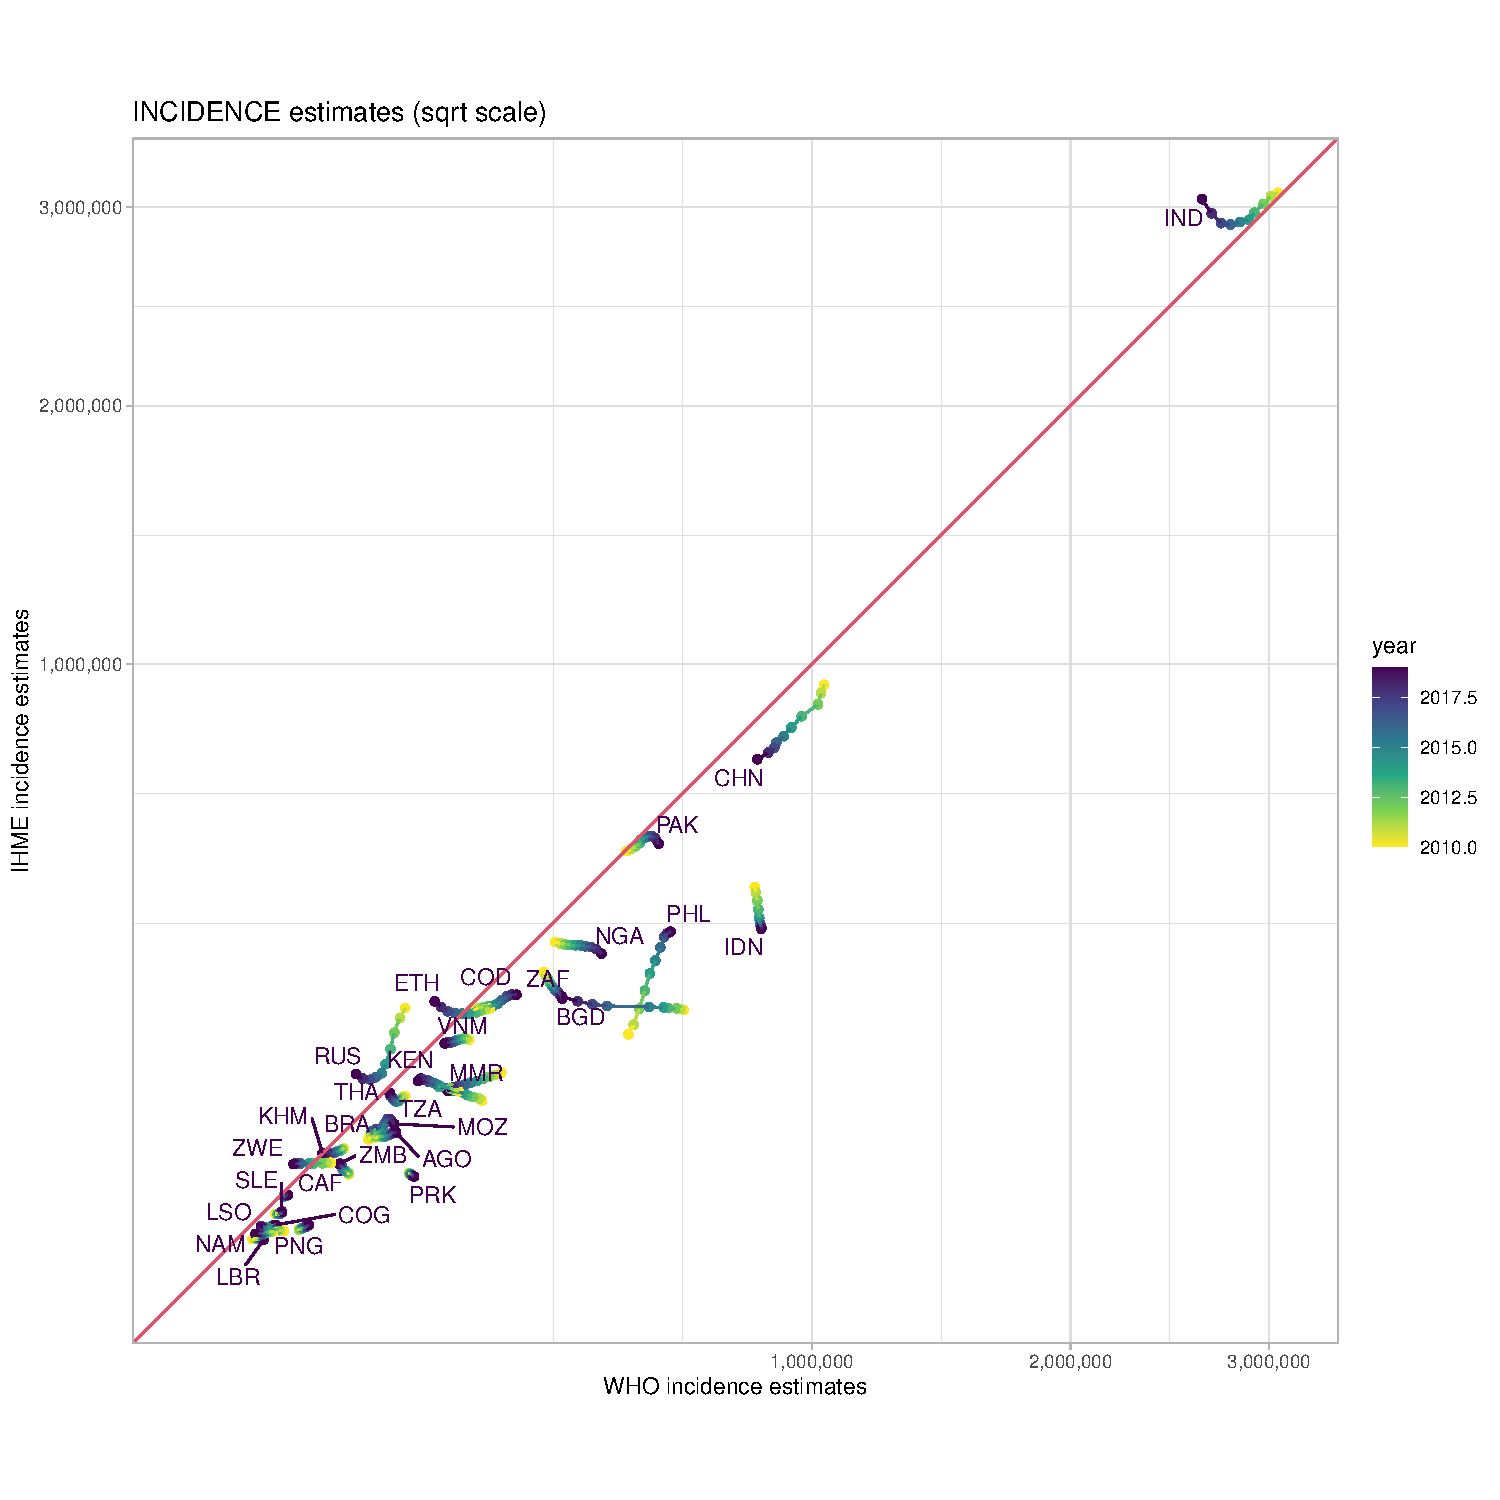
\includegraphics[width=1\textwidth]{../plots/aF2a.pdf}
  \caption[Incidence comparison over time]{Incidence comparison over time. The
    red line represents equality. Percentages are the magnitudes of relative differences
    relative to WHO in 2019.}
\end{figure}


\FloatBarrier

\begin{figure}
  \centering
  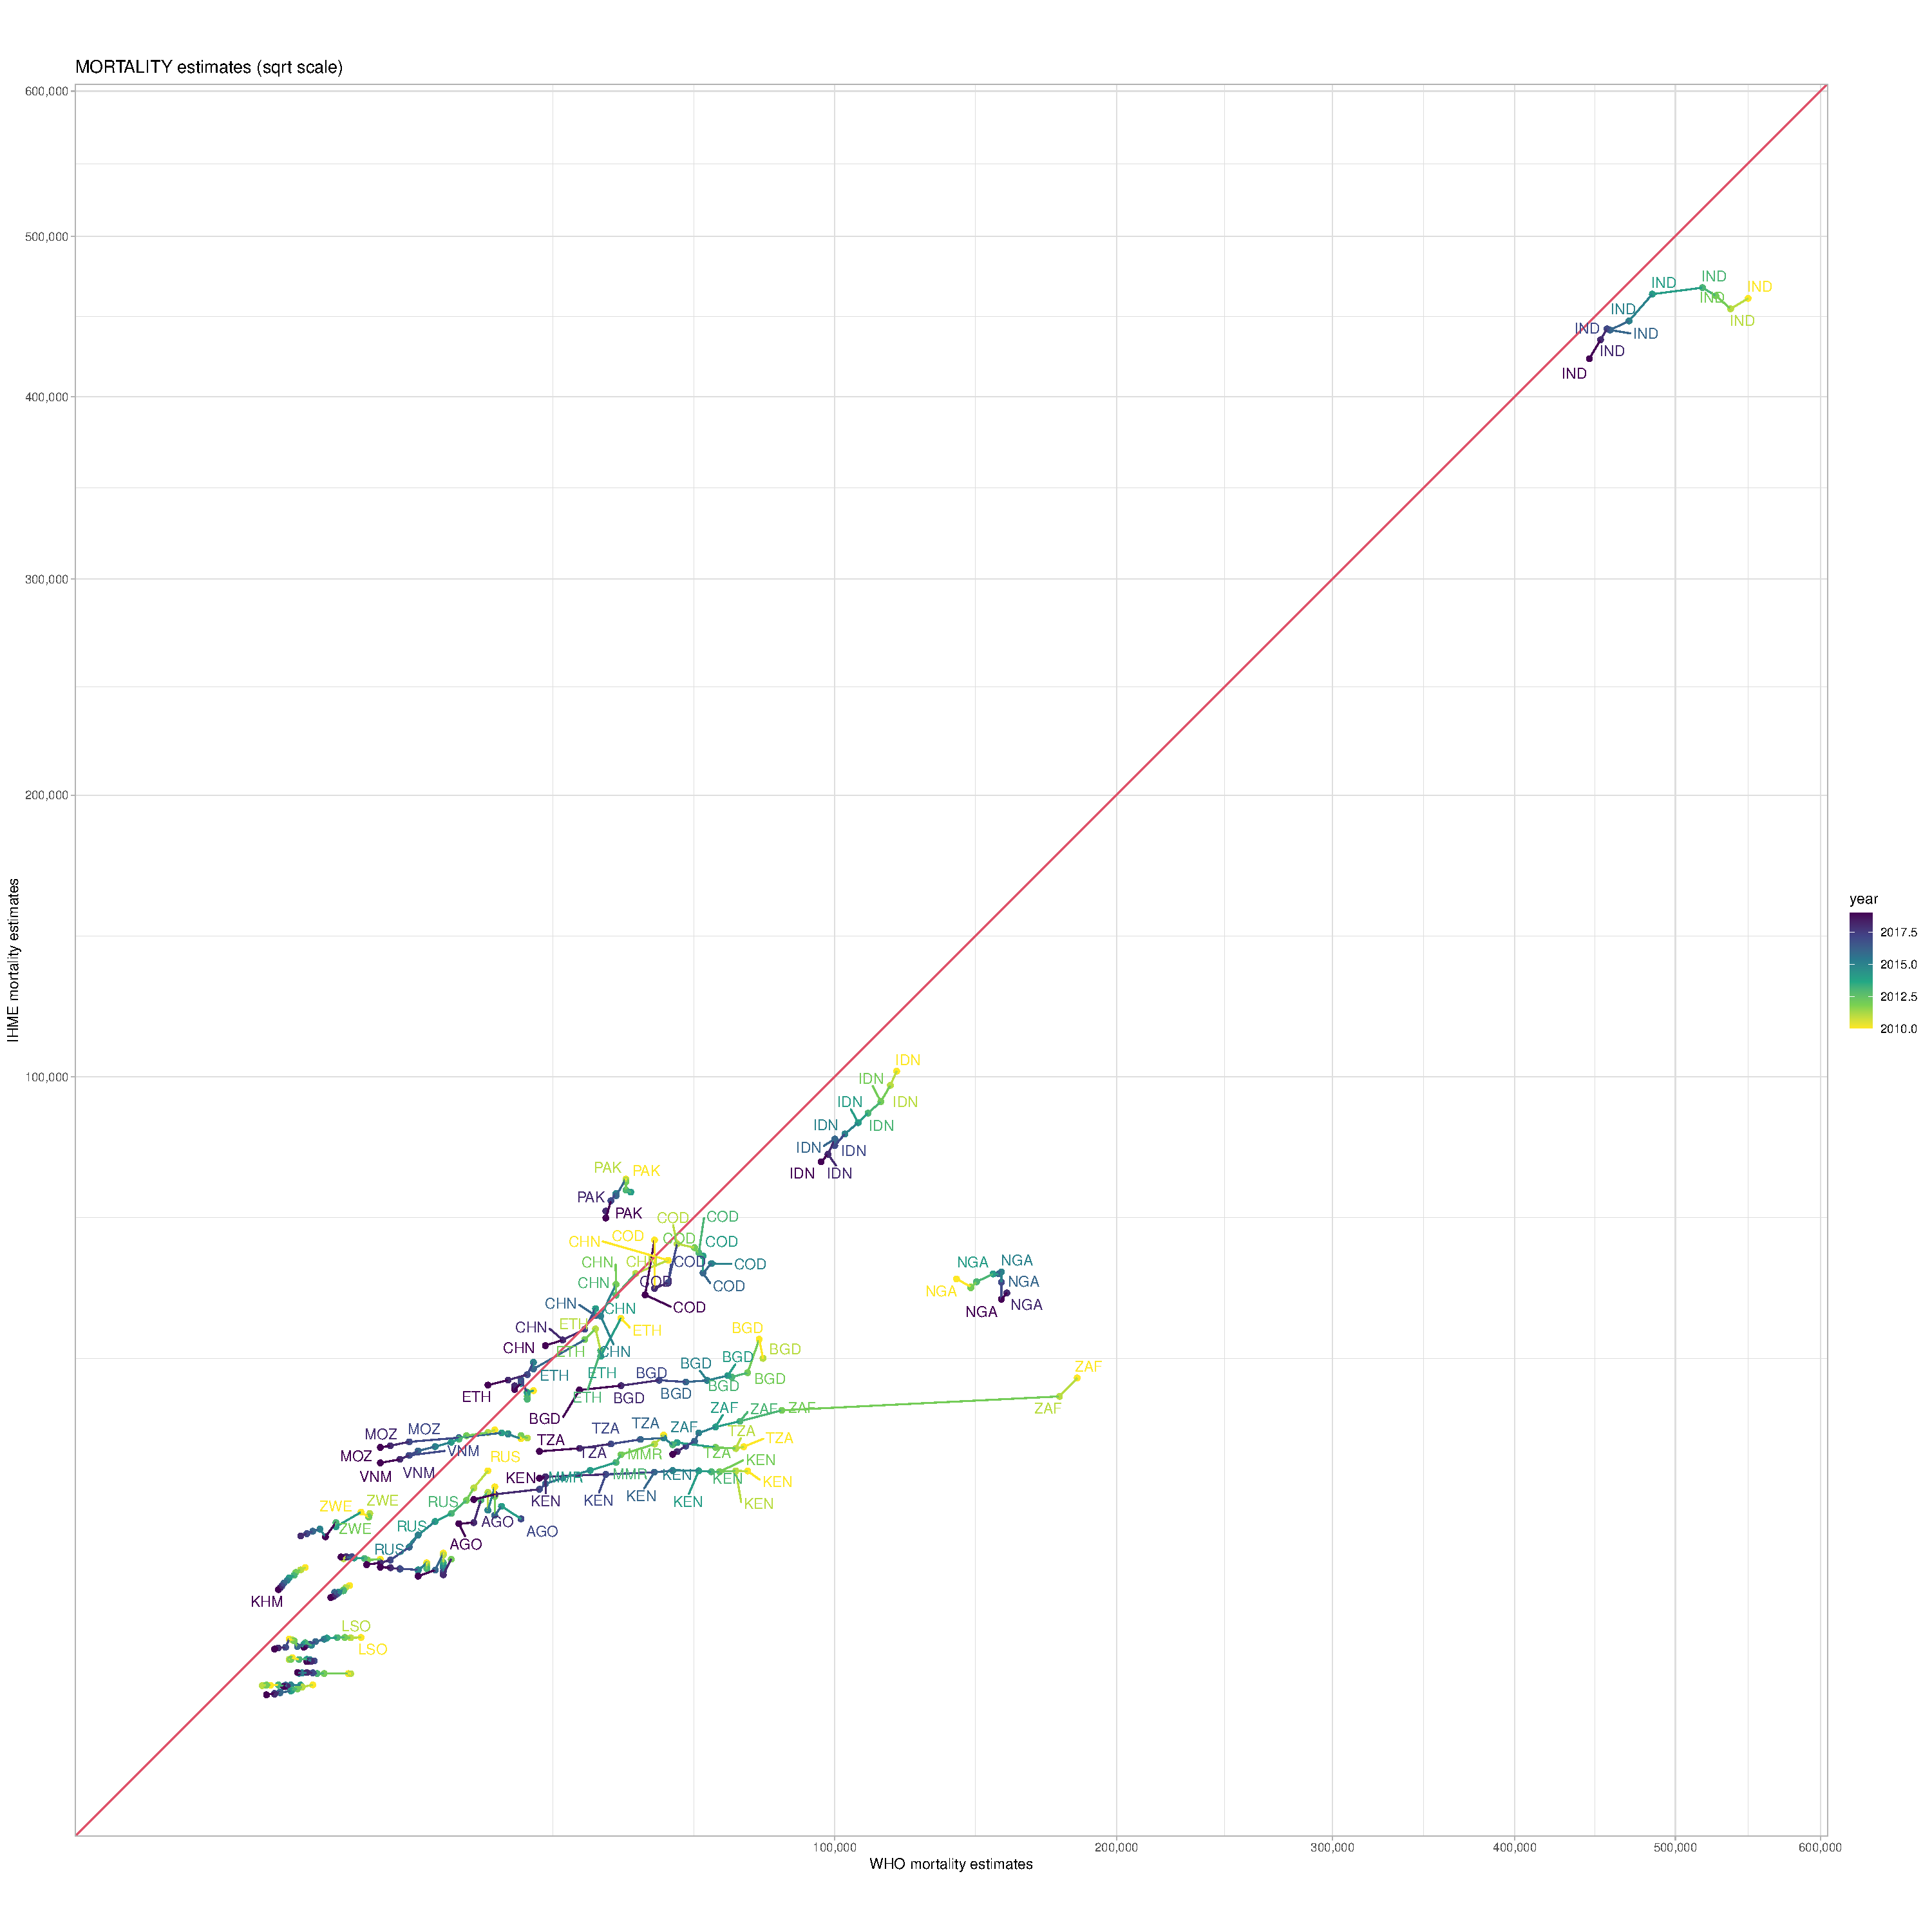
\includegraphics[width=1\textwidth]{../plots/aF2b.pdf}
  \caption[Mortality comparison over time]{Mortality comparison over time. The
    red line represents equality. \\ Percentages are the magnitudes of relative differences
    relative to WHO in 2019.}
\end{figure}

\FloatBarrier

\begin{figure}
  \centering
  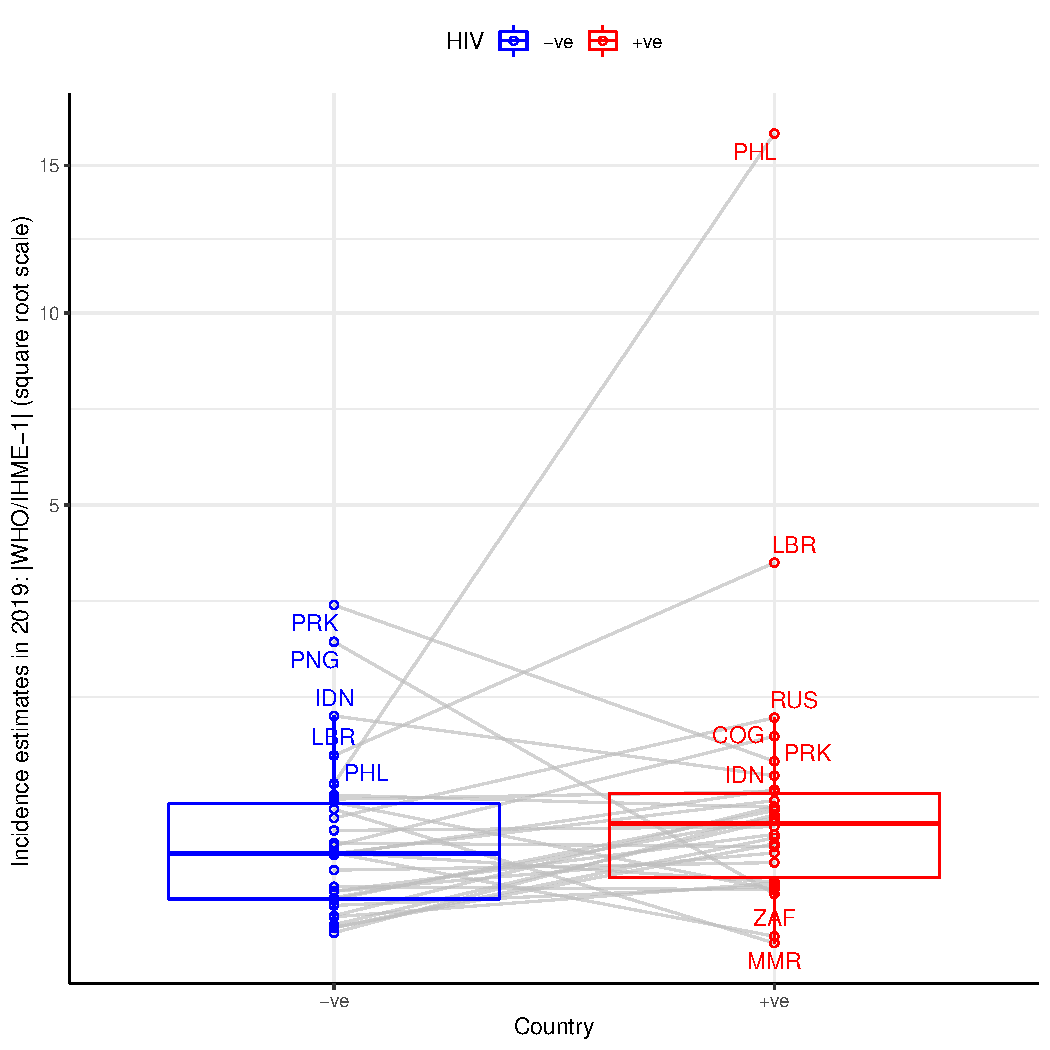
\includegraphics[width=1\textwidth]{../plots/aF9.pdf}
  \caption[WHO vs IHME incidence differences by HIV status]{WHO vs IHME
    incidence differences by HIV status. The difference is the absolute
    difference as a fraction of the IHME estimate. Lines join country HIV$\pm$
    values. Some outlying countries are labelled.}
\end{figure}

\FloatBarrier


\begin{figure}
\centering
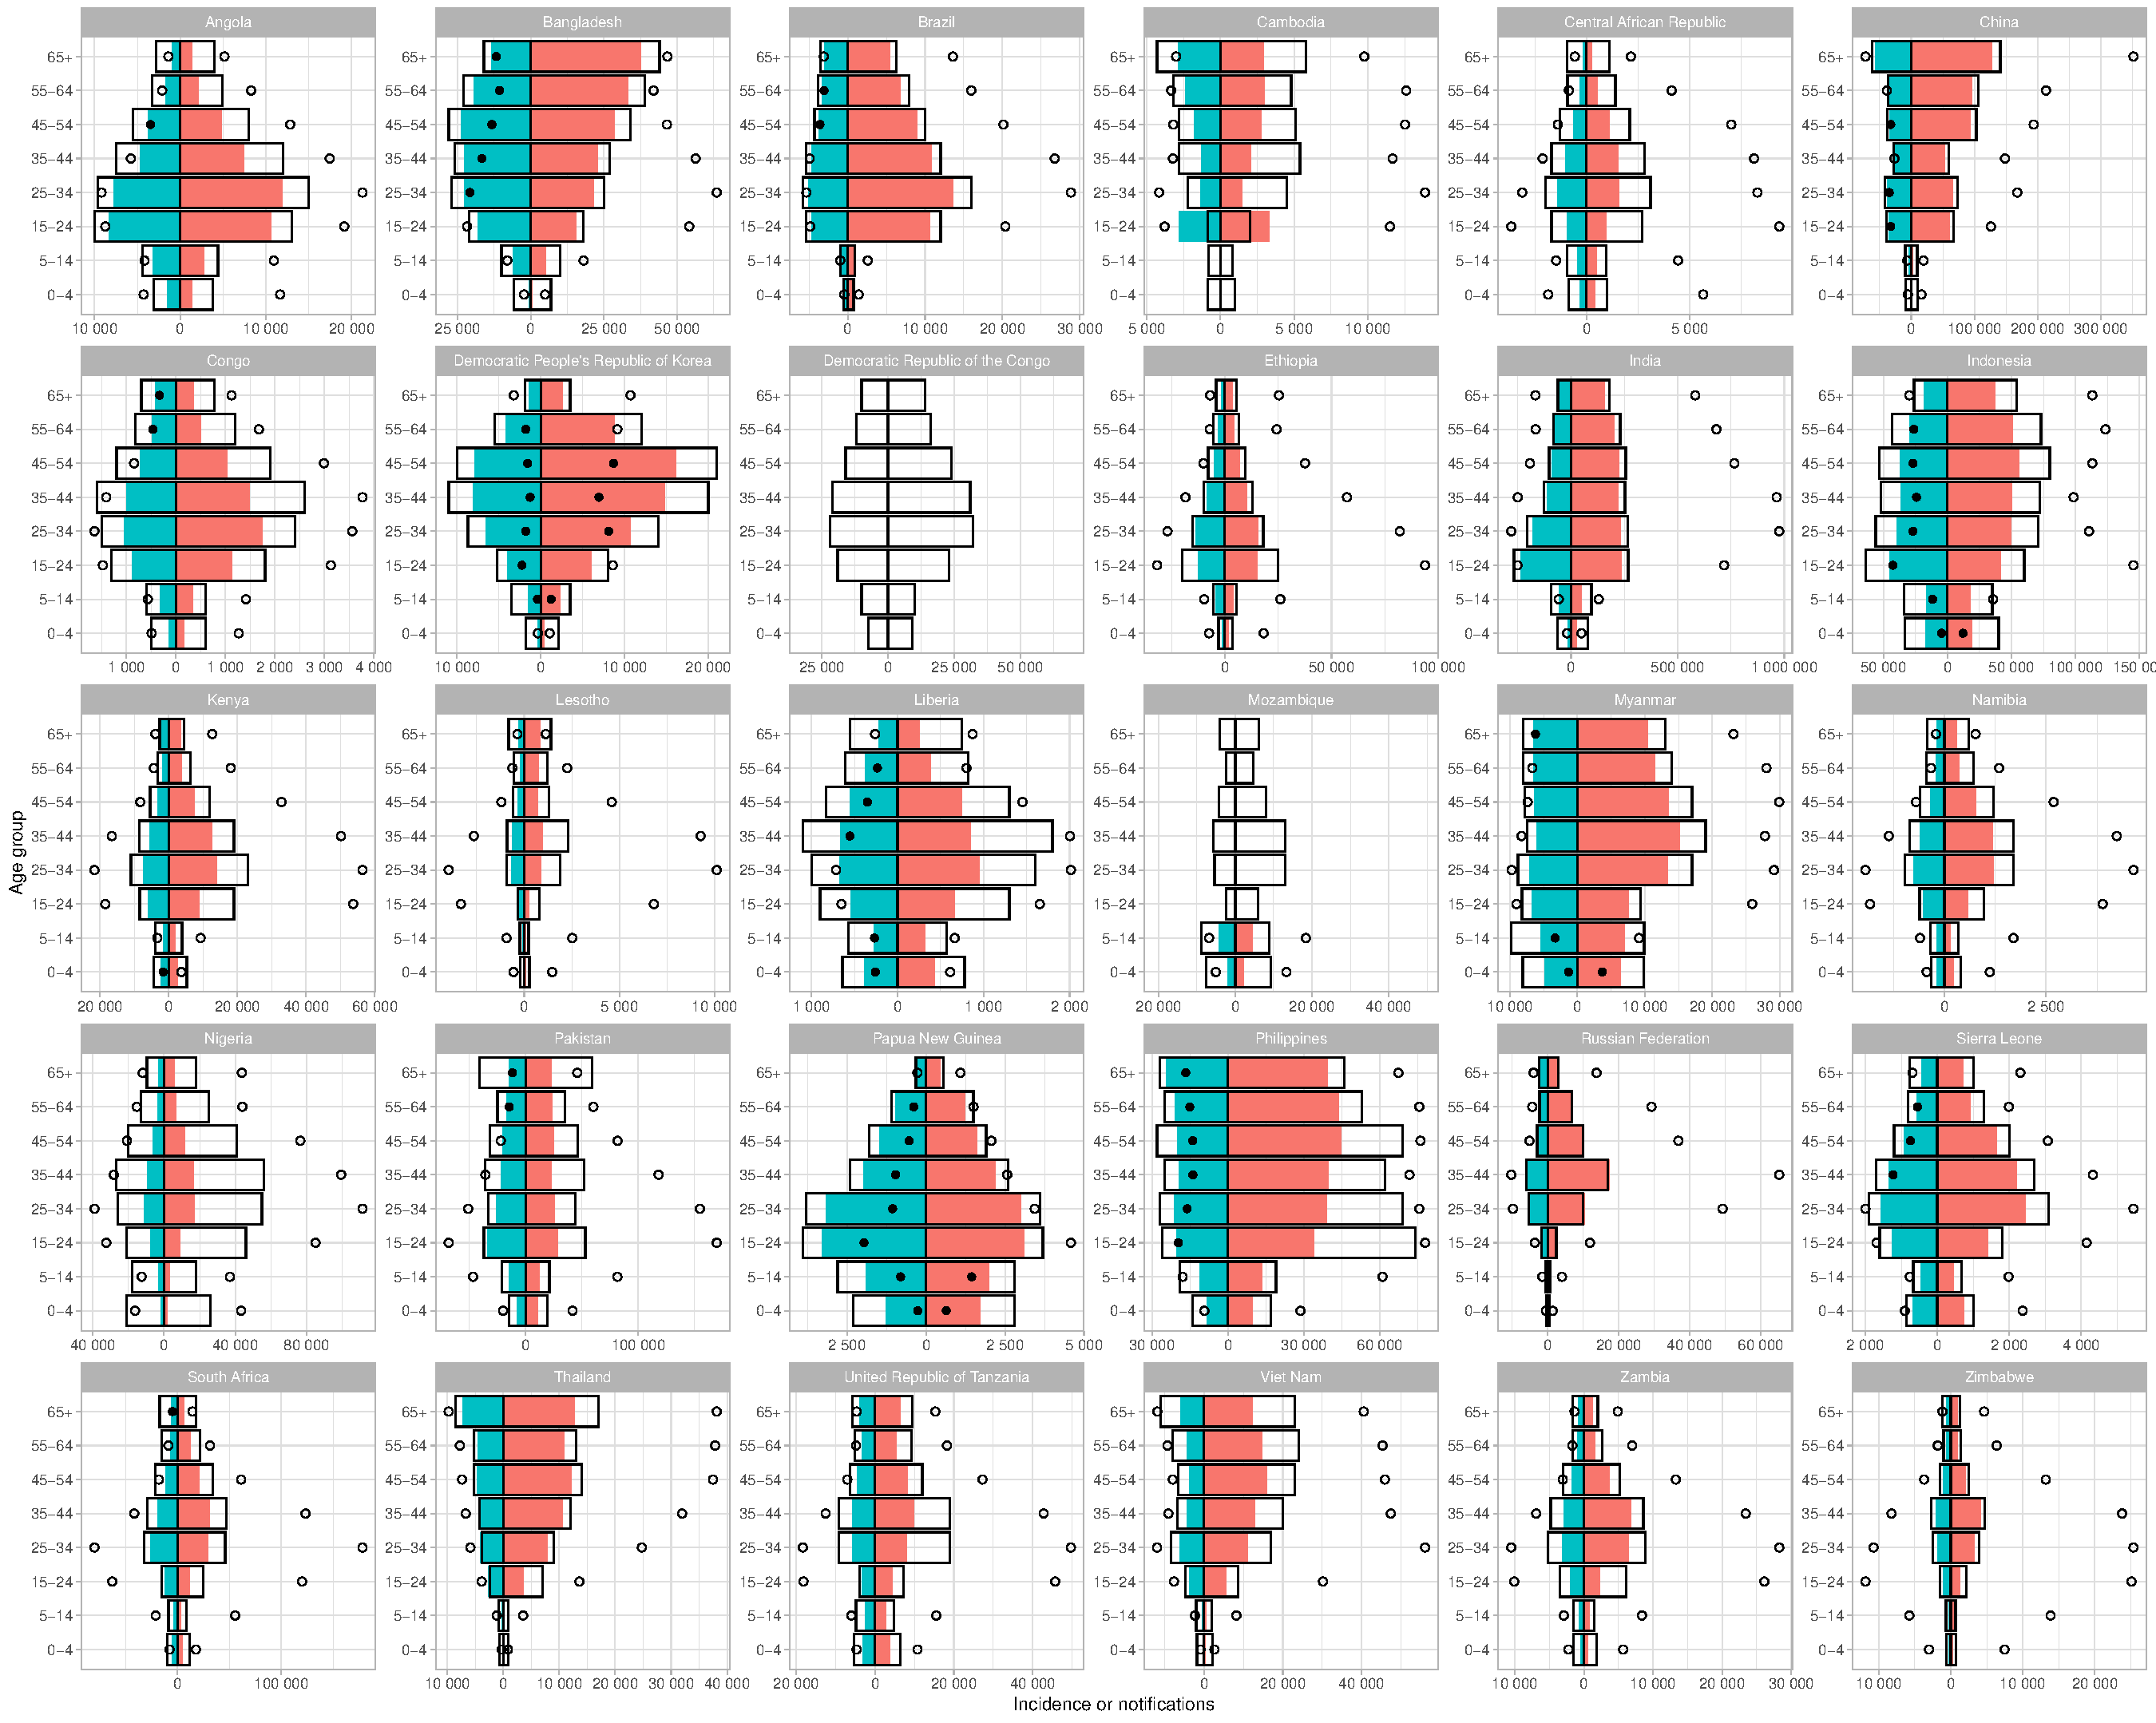
\includegraphics[width=1\textwidth]{../plots/aF1.pdf}
\caption[30 HBC incidence and notifications]{30 HBC incidence and notifications
  for 2019.
  Coloured bars are notifications; open bars are WHO incidence estimates; circles are IHME GBD incidence estimates, where filled circles suggest a case detection ratio greater than one according to these estimates. Men to the right; women to the left.}
\end{figure}


\FloatBarrier


% \begin{figure}
%   \centering
%   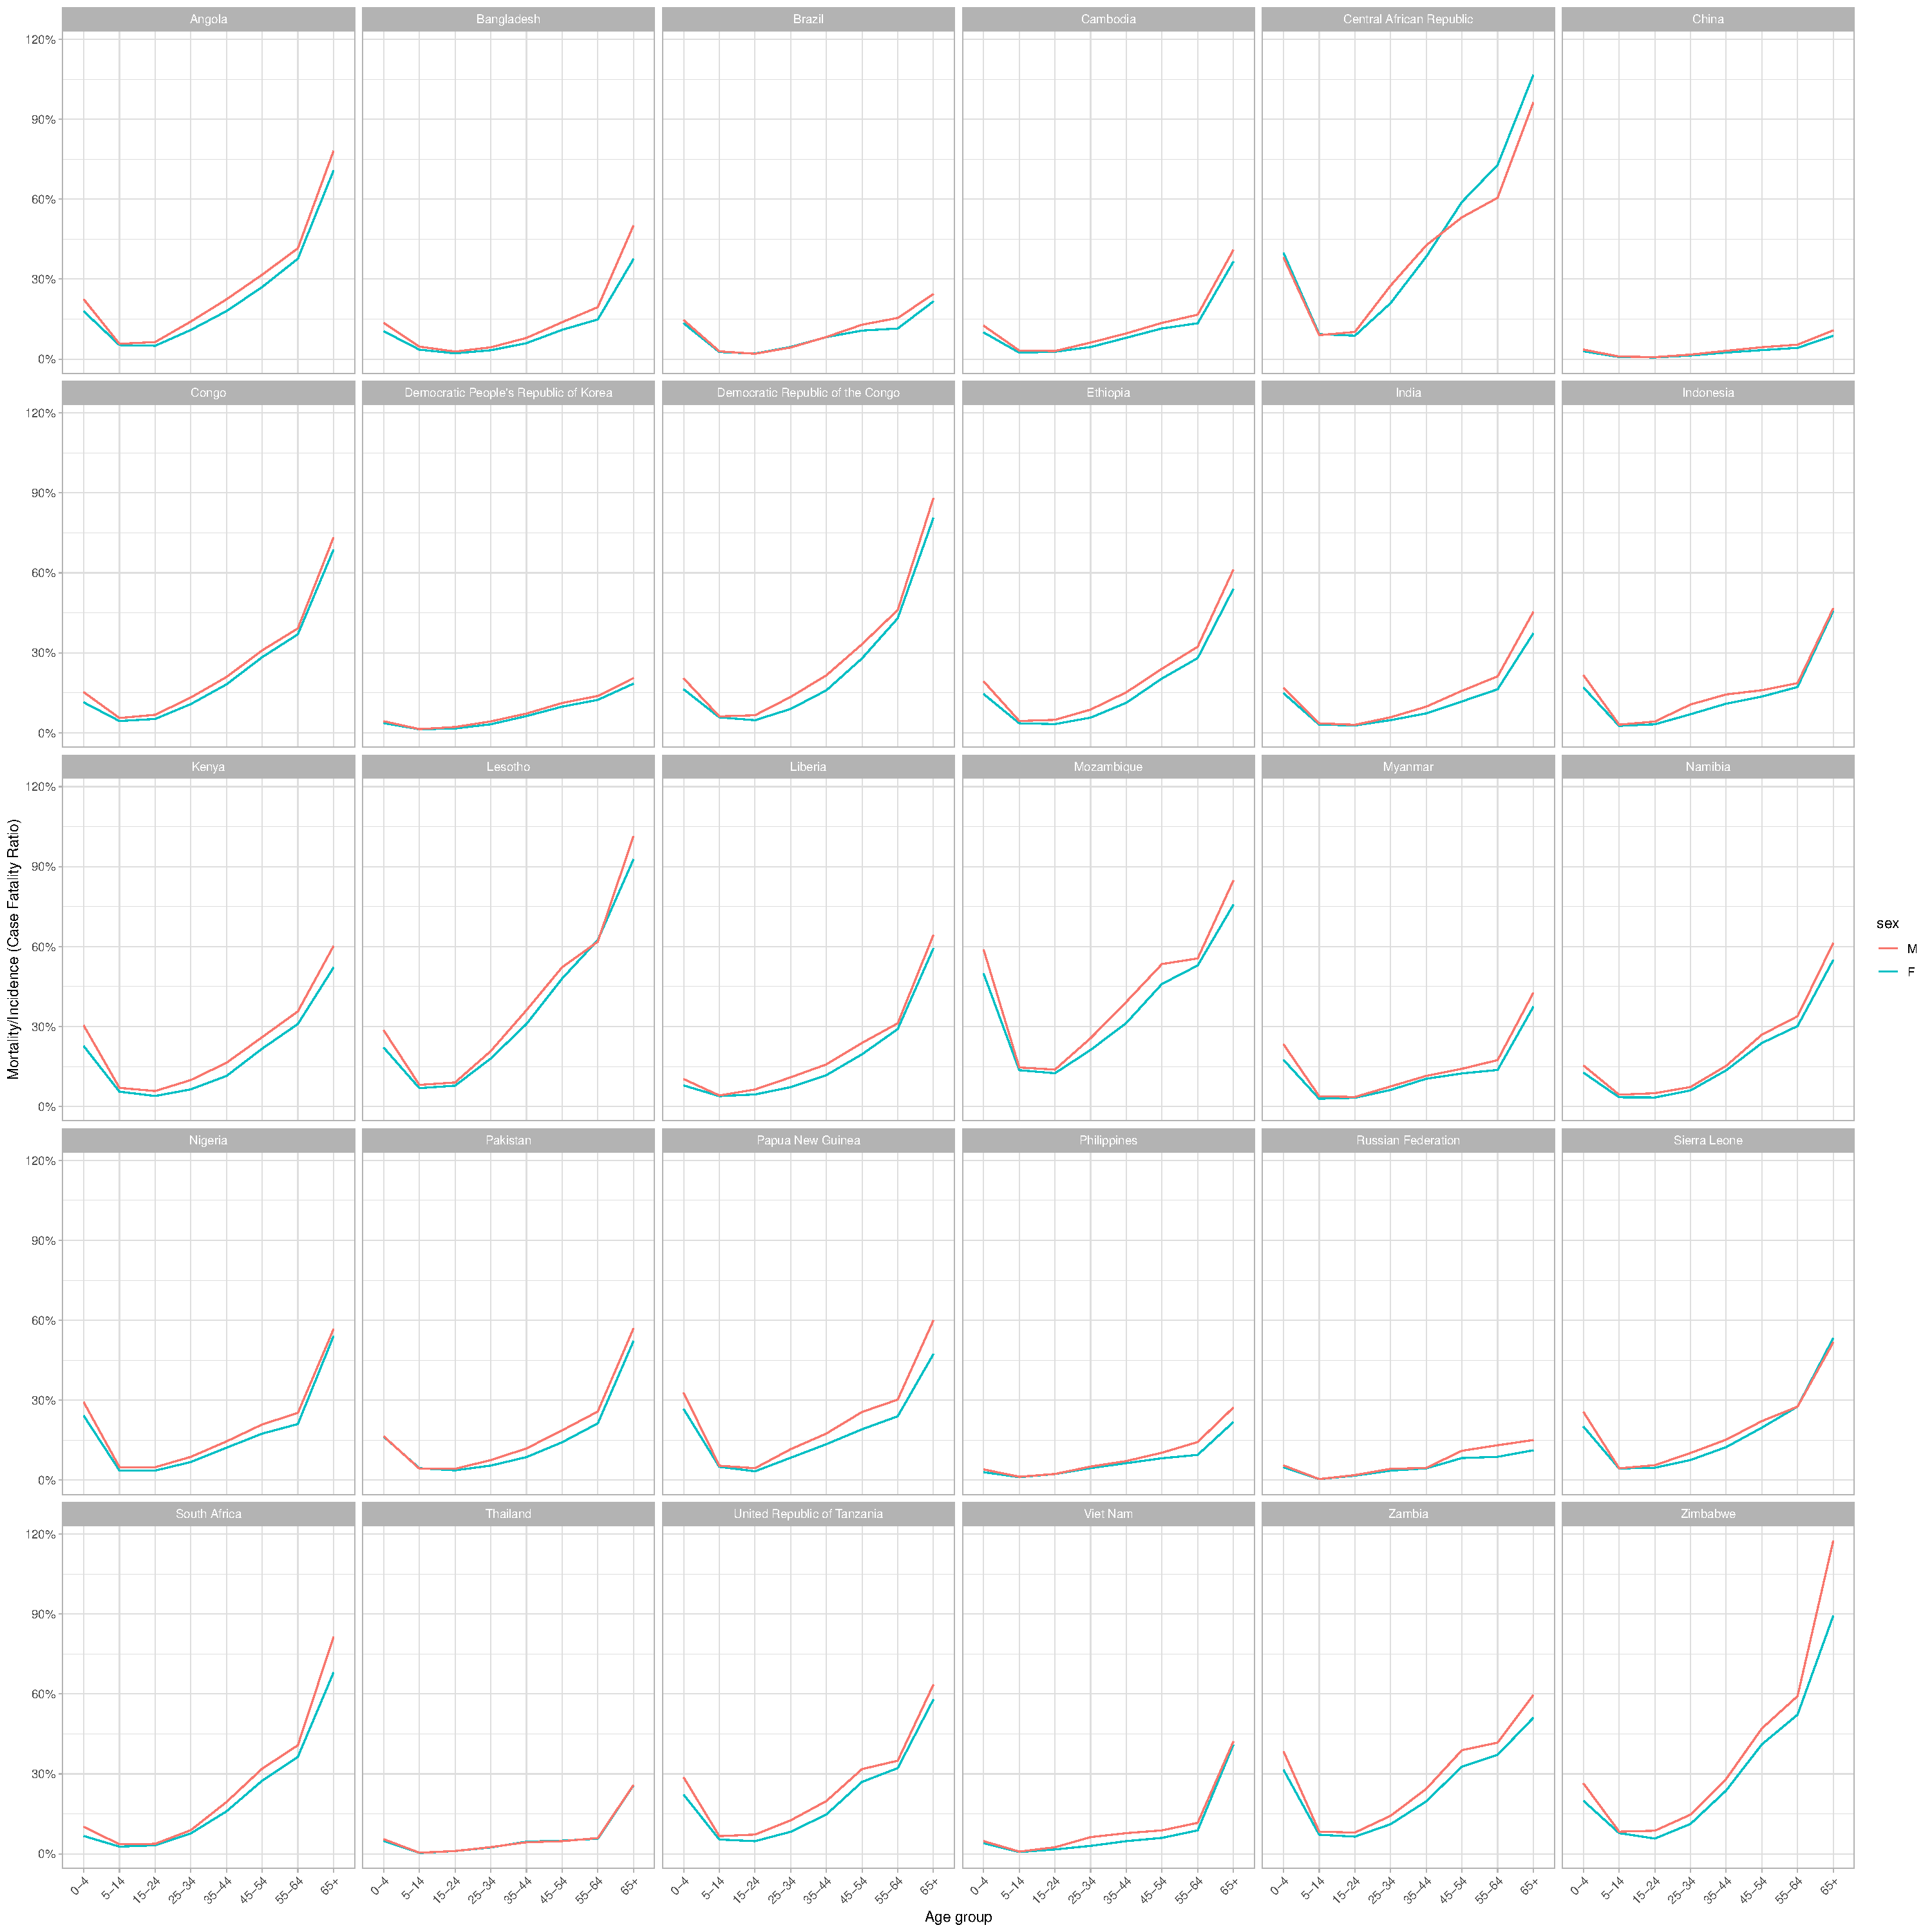
\includegraphics[width=1\textwidth]{../plots/aF4.pdf}
%   \caption[Case Fatality Ratio by age and sex]{Case Fatality Ratio (CFR) by age and
%     sex. CFR is calculated as estimated mortality over esimtated incidence in 2019}
% \end{figure}


\FloatBarrier

\begin{figure}
\centering
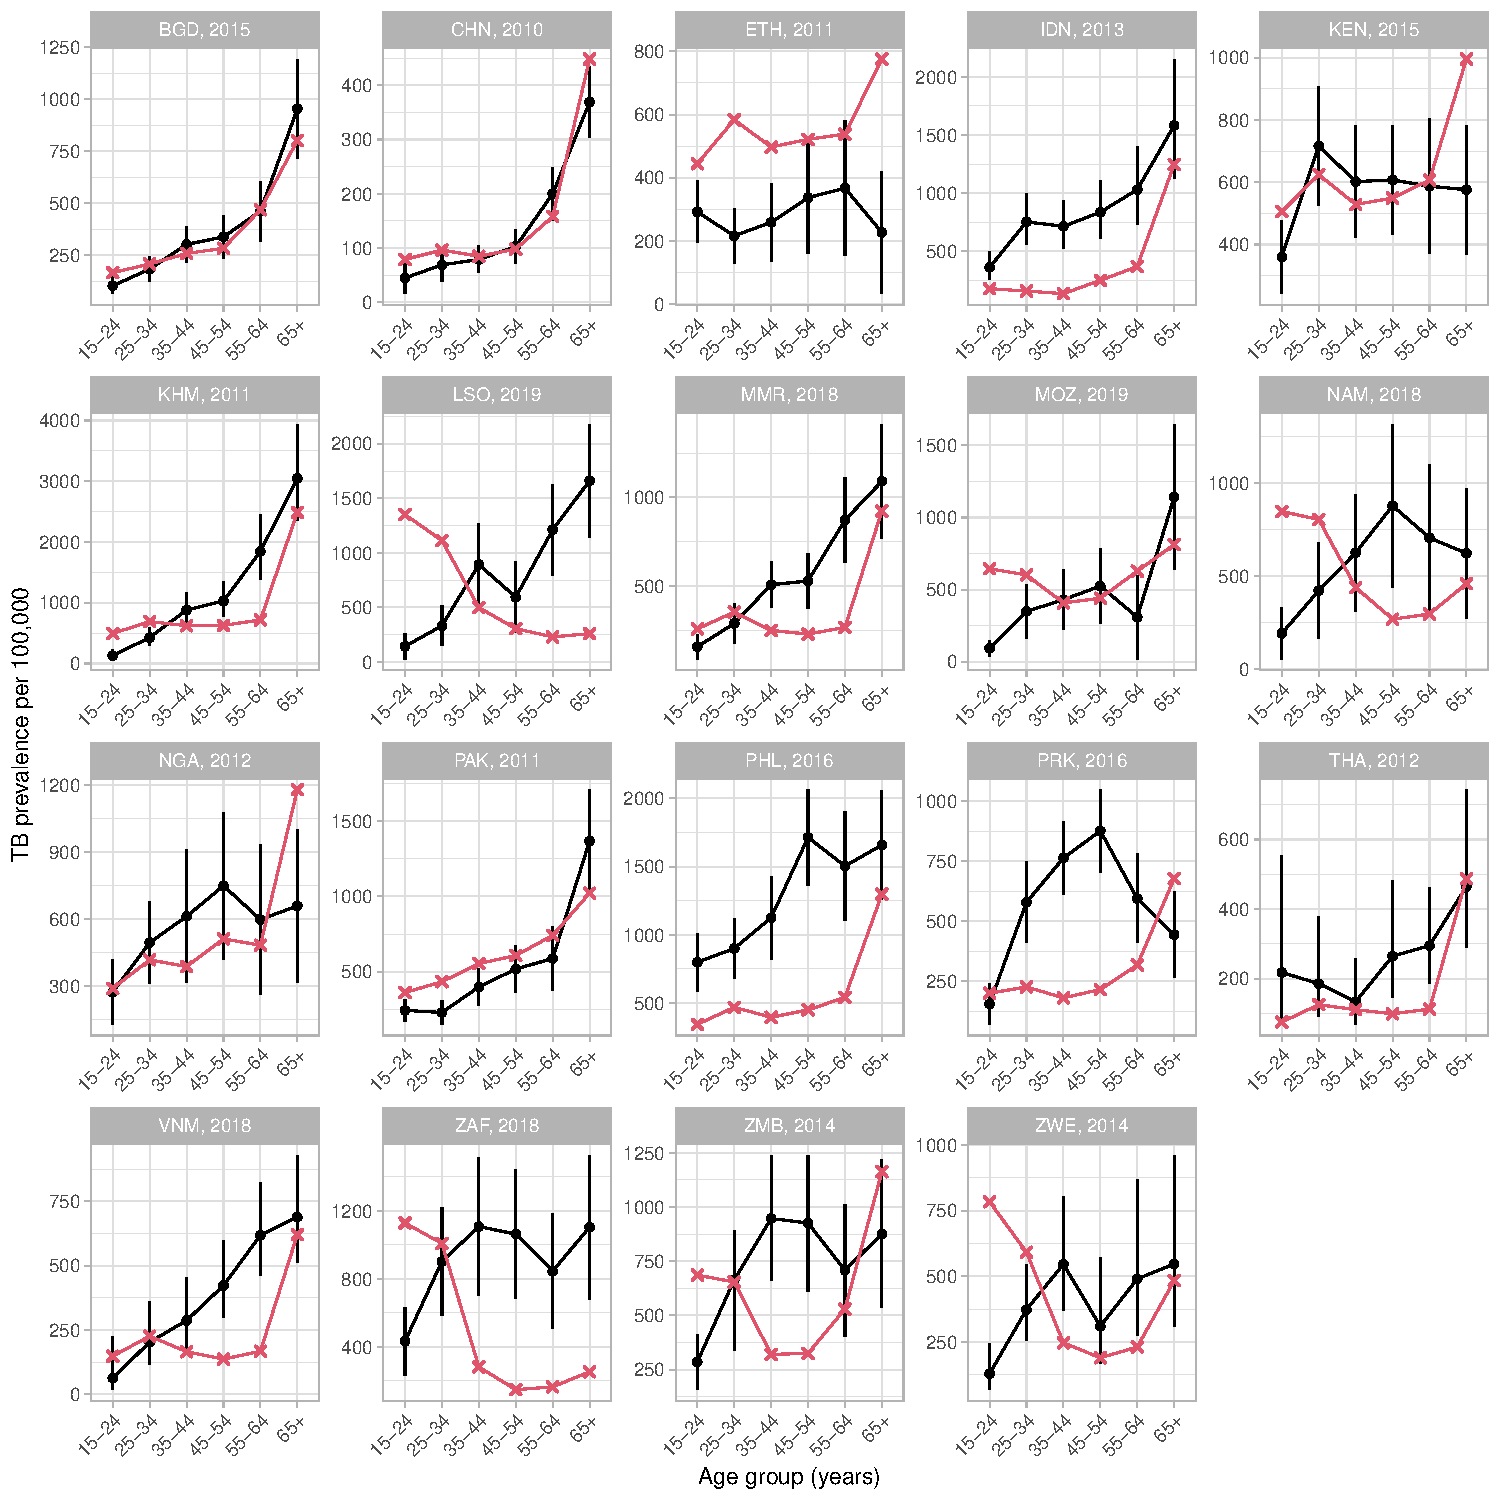
\includegraphics[width=1\textwidth]{../plots/aF3.pdf}
\caption[Prevalence vs prevalence survey.]{Prevalence vs
  nationally-representative prevalence survey. Red=IHME all TB prevalence point
  estimate; black=prevalence survey bacteriologically-confirmed TB prevalence
  and 95\% confidence interval. Bacteriologically-confirmed TB is a subset of
  all TB.}
\end{figure}

\FloatBarrier

\begin{figure}
  \centering
  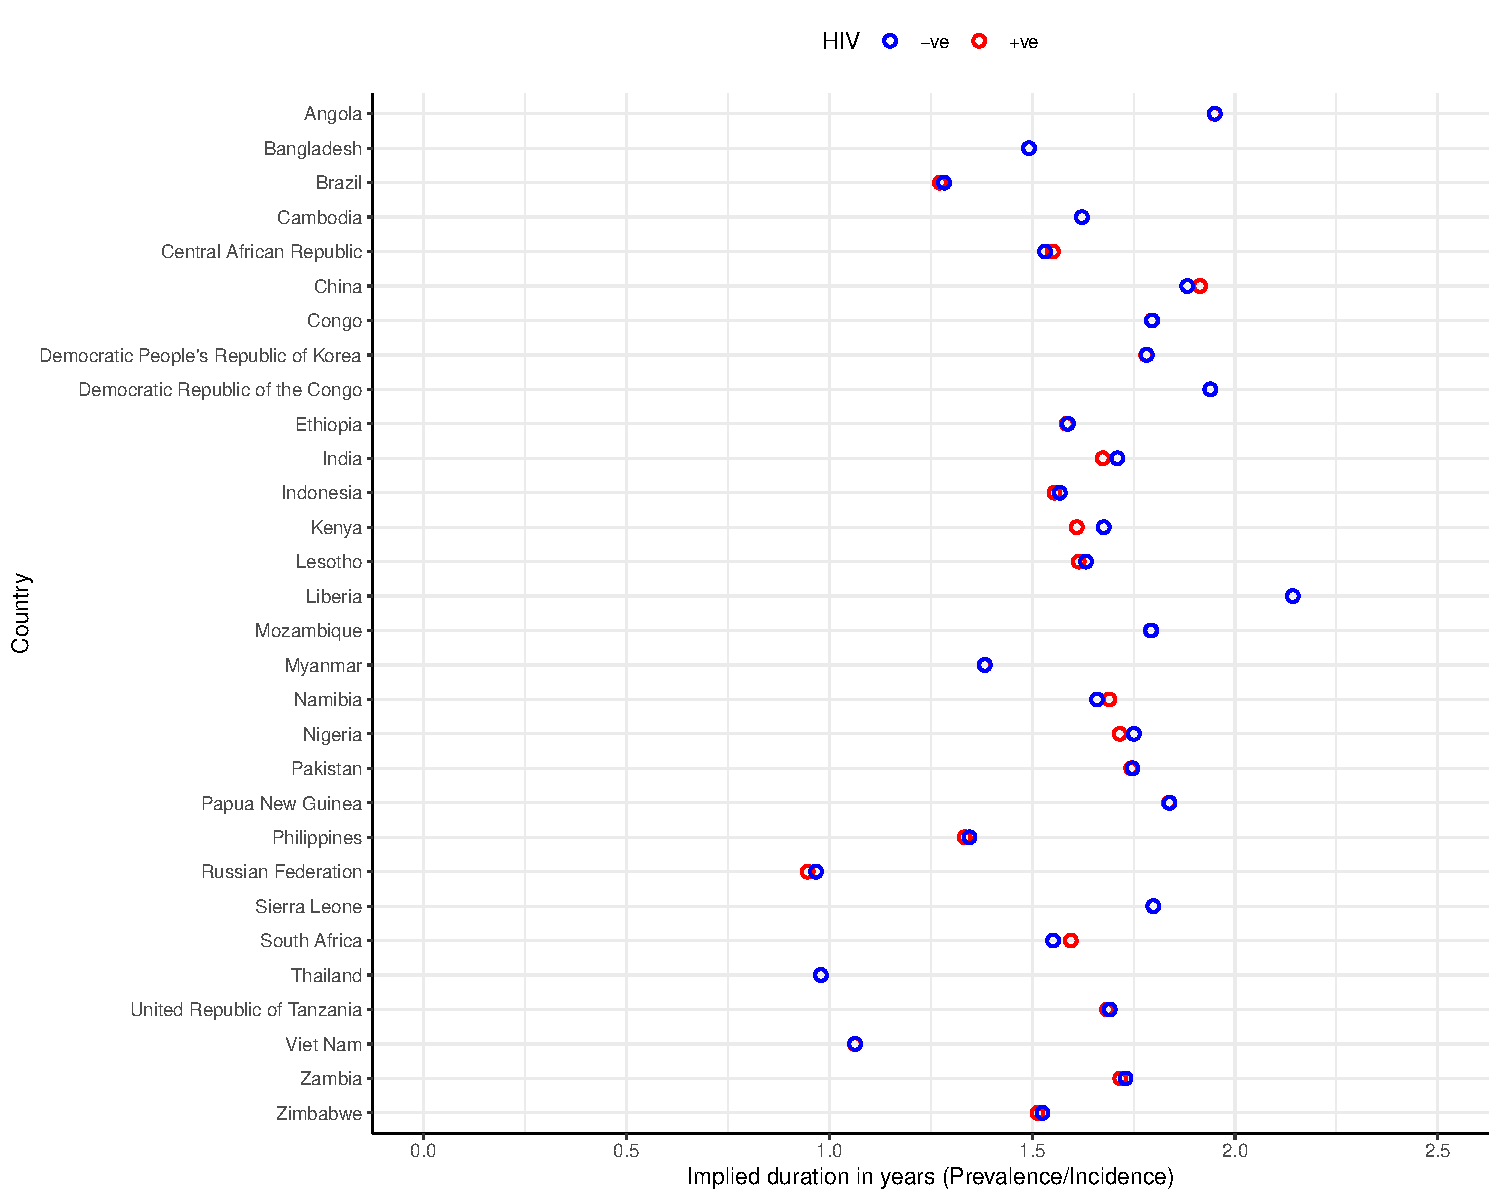
\includegraphics[width=1\textwidth]{../plots/aF7.pdf}
  \caption[Implied duration by HIV status]{Implied duration by HIV status.
    Duration is calculated as estimated prevalence divided by estimated
    incidence. HIV-associated TB is thought to have shorter duration than TB
    disease in HIV uninfected people. Some red (HIV+) and blue (HIV-) points are not
    distinguishable due to overlap.}
\end{figure}


\FloatBarrier


\begin{figure}
  \centering
  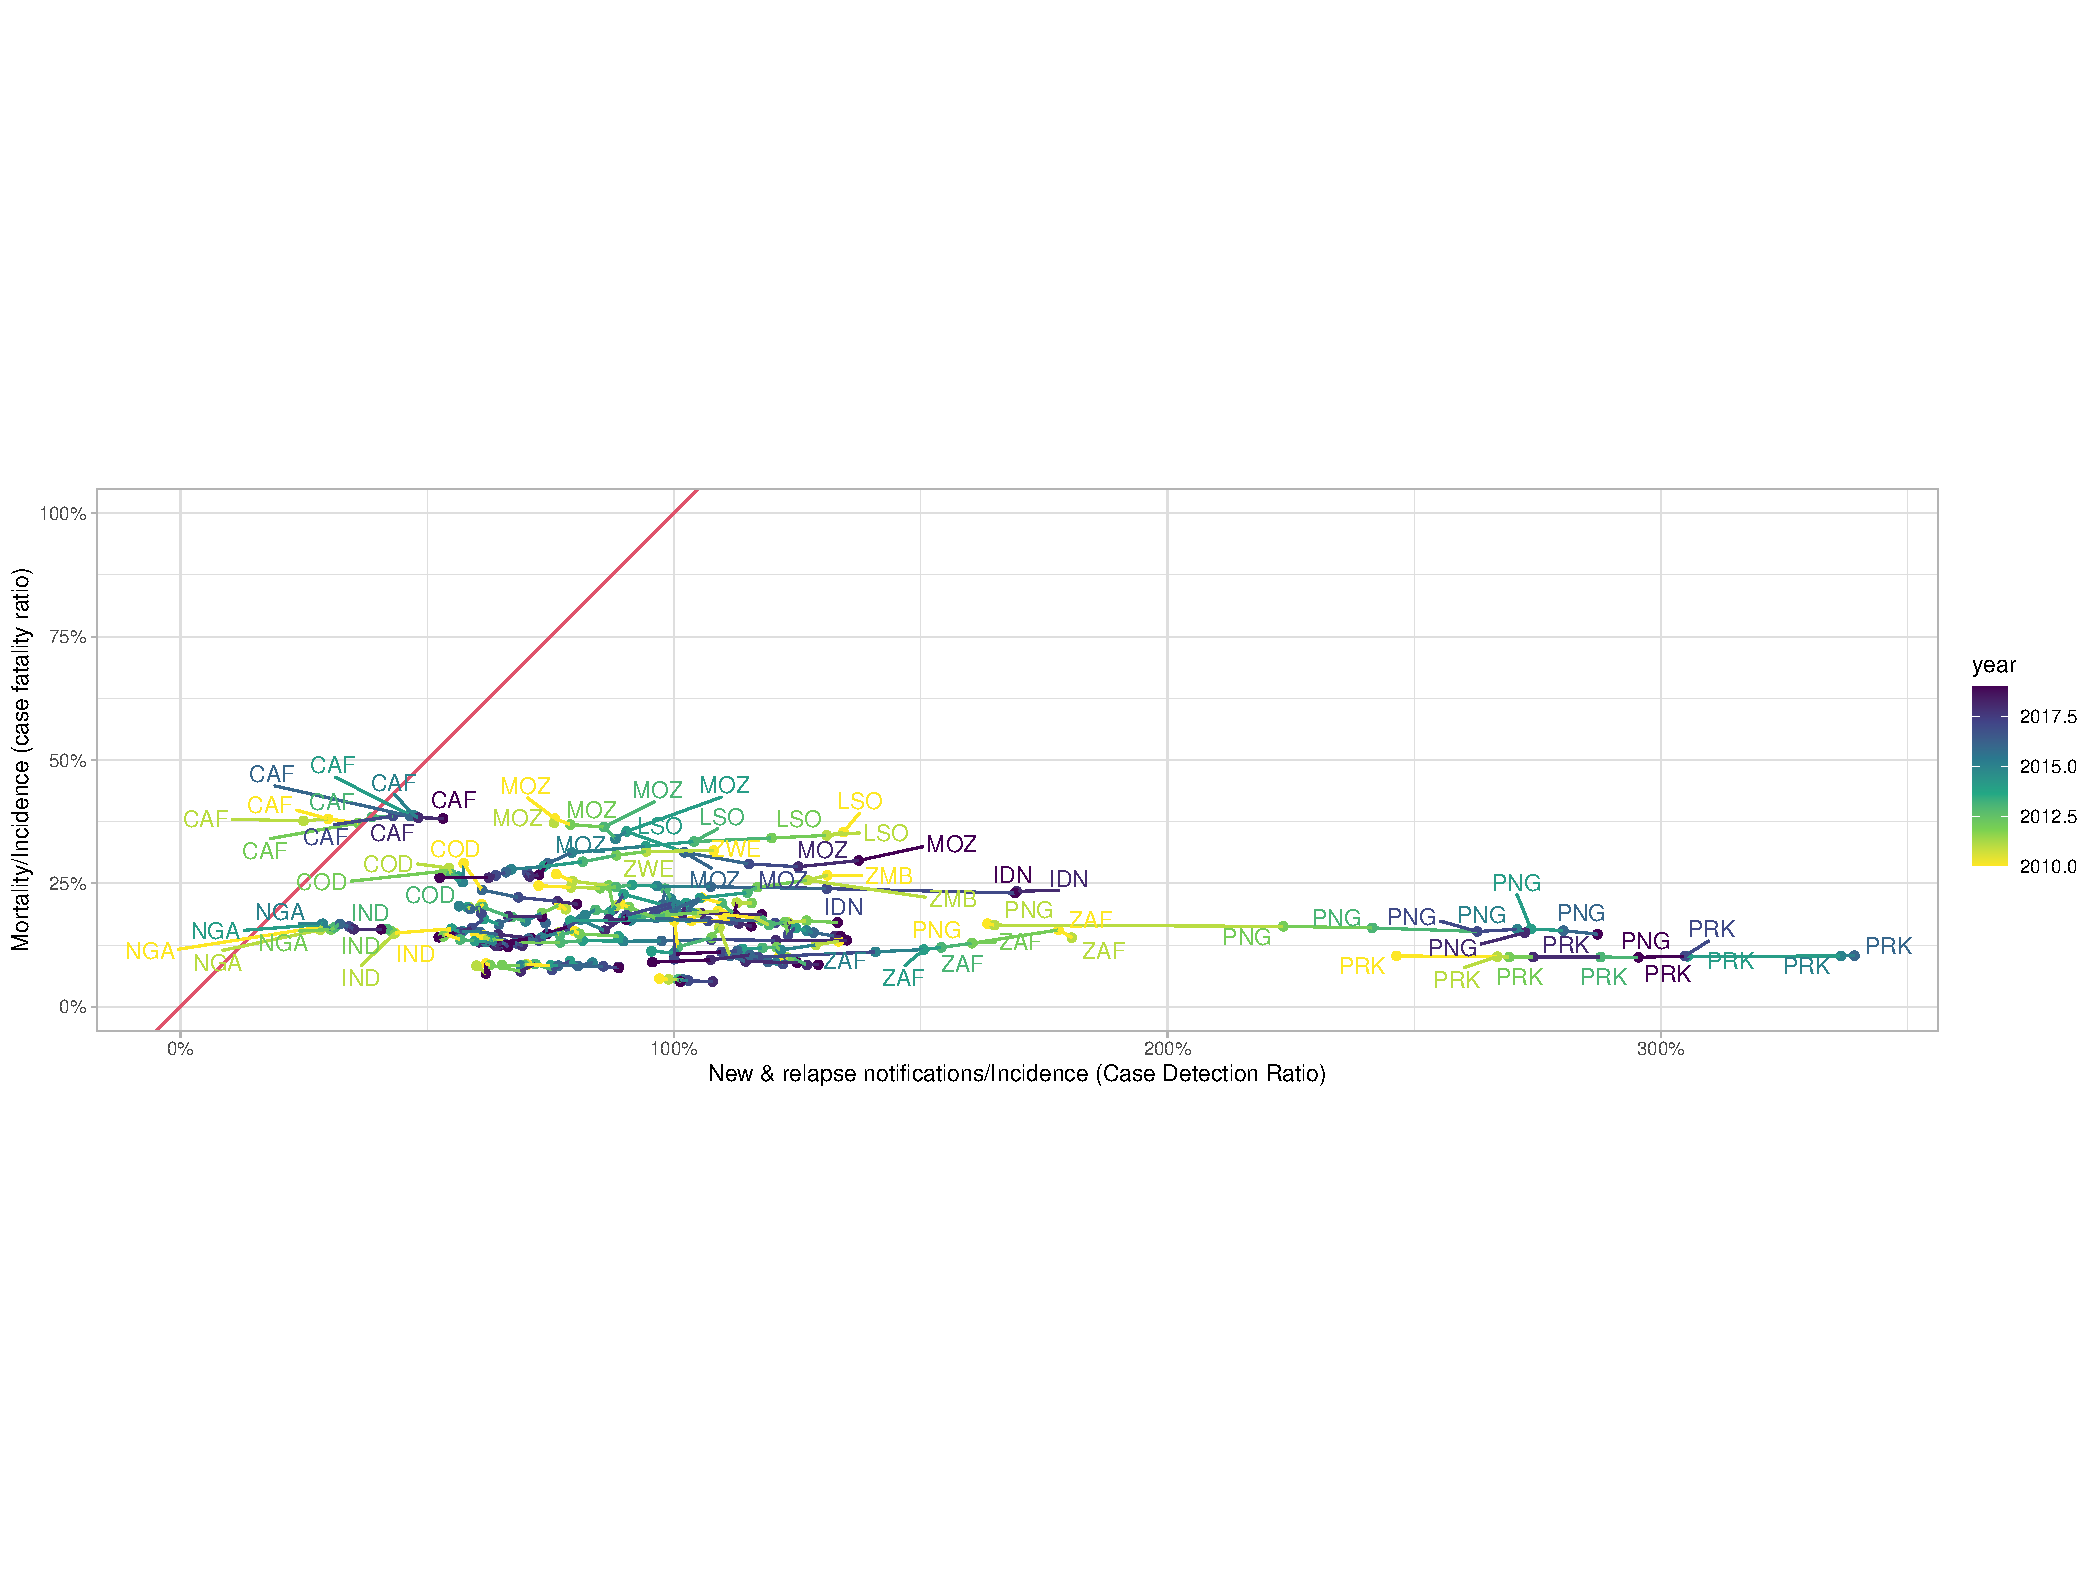
\includegraphics[width=0.8\textwidth]{../plots/aF8.pdf}
  \caption[Case Fatality Ratio vs Case Detection Ratio]{IHME Case Fatality Ratio vs
    Case Detection Ratio 2010-2019. Case Fatality Ratio (CFR) is calculated as estimated
    mortality divided by estimated incidence.
    Case Detection Ratio (CDR) is calculated as notifications divided by
    estimated incidence. The red diagonal line is a reference line of equality.
    The horizontal grey line represents a CDR of 100\%. CFRs are typically
    stable even for large changes in CDR.}
\end{figure}

\FloatBarrier

\begin{figure}
\centering
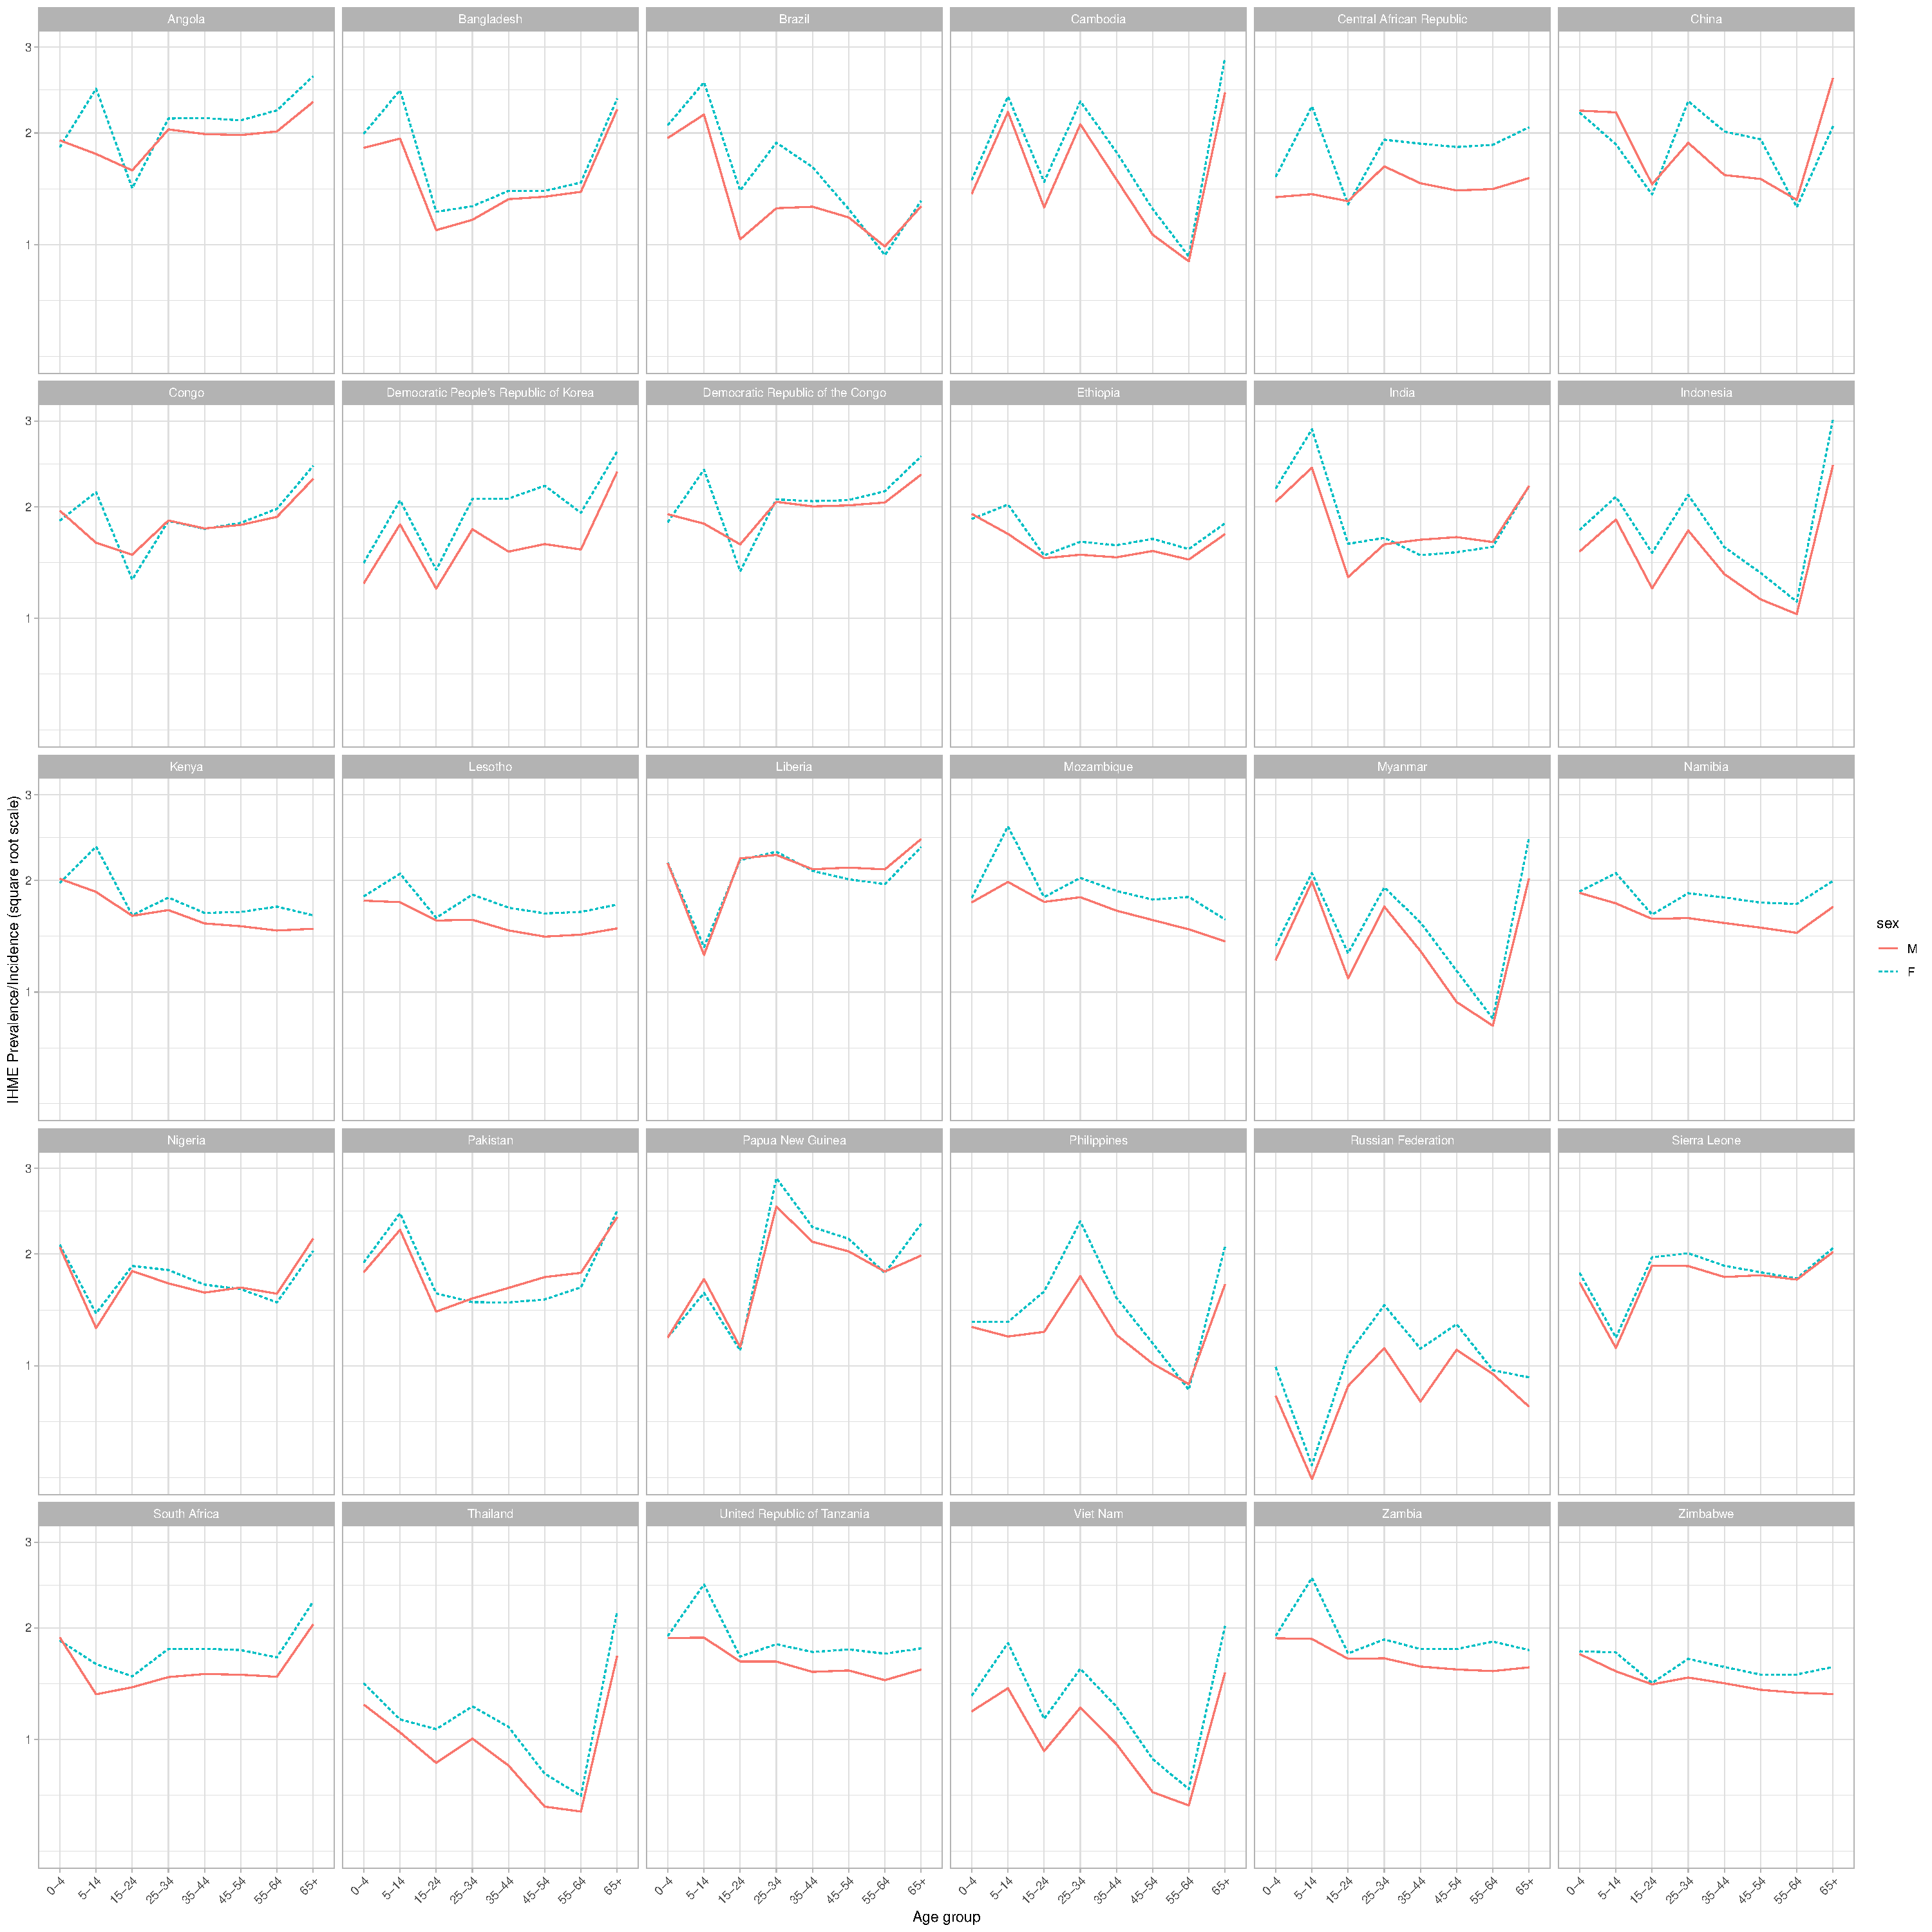
\includegraphics[width=1\textwidth]{../plots/aF5.pdf}
\caption[Implied duration by age and sex]{Implied duration by age and sex.
  Duration is calculated as estimated prevalence divided by estimated incidence.
The y-axis is on a square root scale. Most settings have similar oveall
duration. Most settings have litte difference in duration by sex.}
\end{figure}

\FloatBarrier

\begin{figure}
\centering
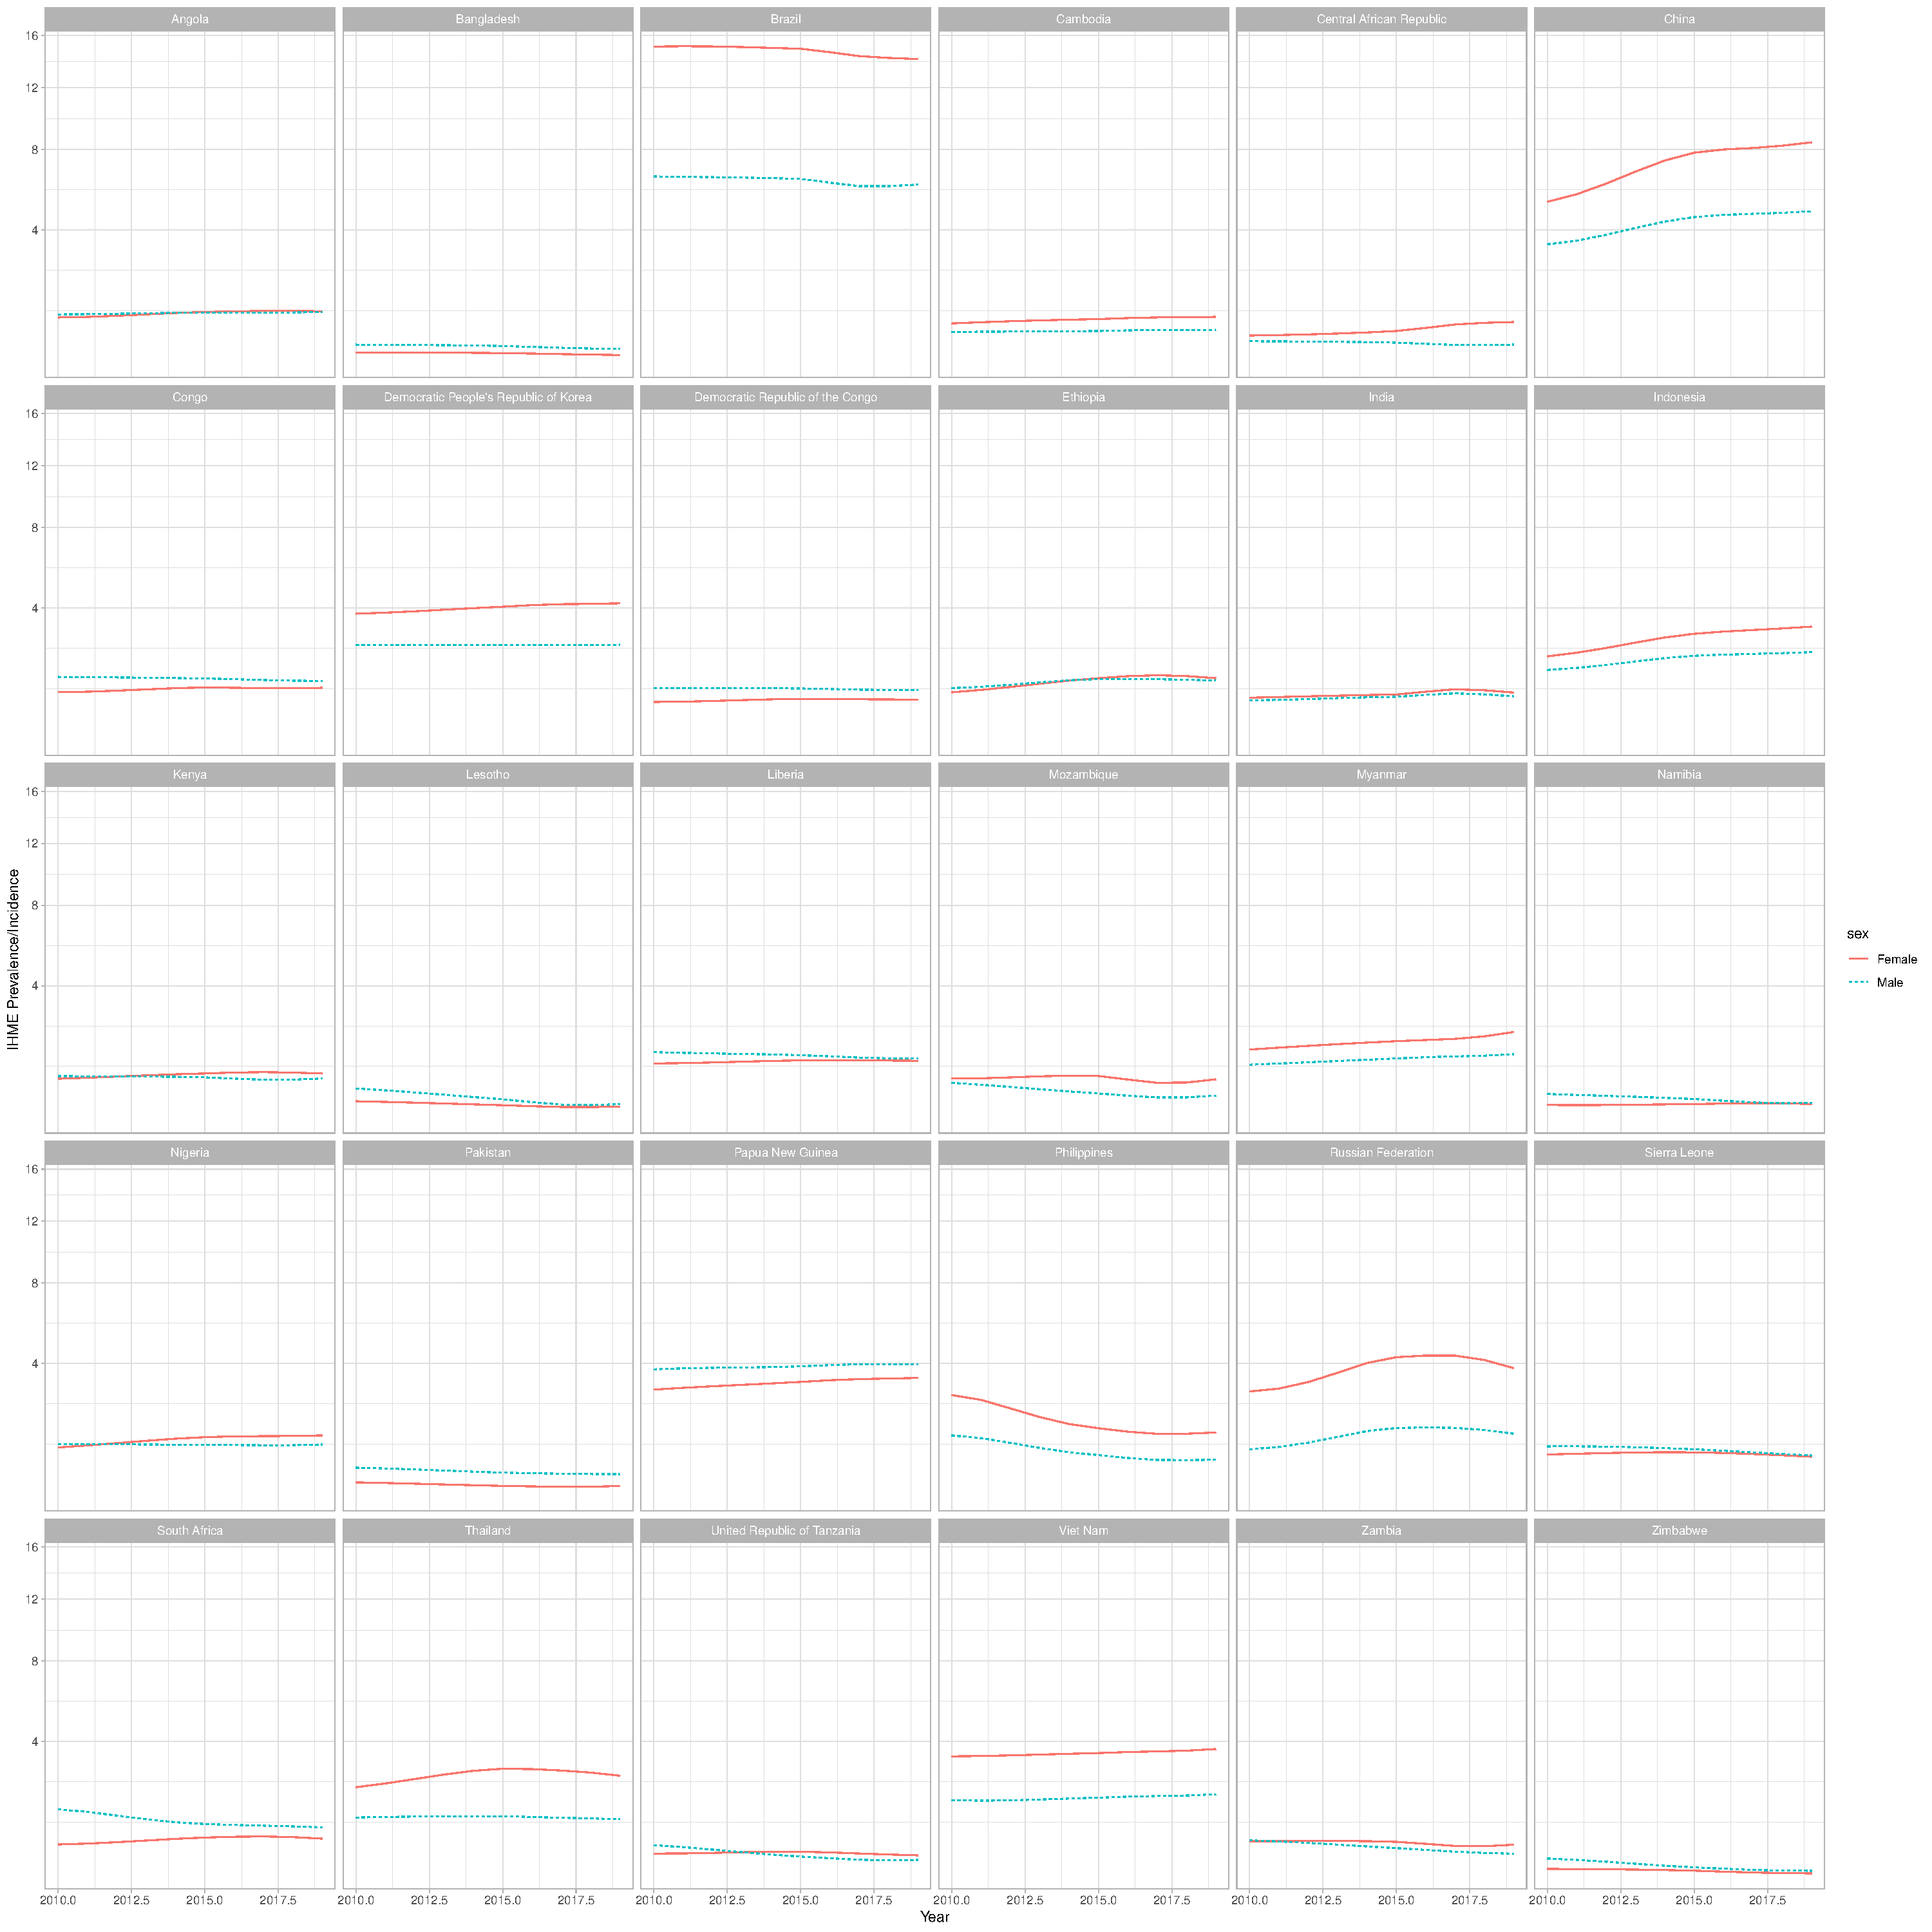
\includegraphics[width=1\textwidth]{../plots/aF6.pdf}
\caption[Implied duration over time]{Implied duration over time. Duration is
  calculated as estimated prevalence divided by estimated incidence. Most
  settings show quite stable durations.}
\end{figure}

\end{document}
